\documentclass[report.tex]{subfiles}

\externaldocument{report}

\begin{document}

\section{原理}

\subsection{ラジオ回路}

\wfig{radio-circuit}にラジオ回路を示す。

\begin{figure}[H]
	\centering
	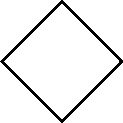
\includegraphics[width=7cm]{fig/radio.pdf}
	\caption{ラジオ回路}
	\label{fig:radio-circuit}
\end{figure}

\subsection{増幅回路}

\wfig{amplifier-circuit}に増幅回路を示す。
\wfig{amplifier-circuit}は、

\begin{figure}[H]
	\centering
	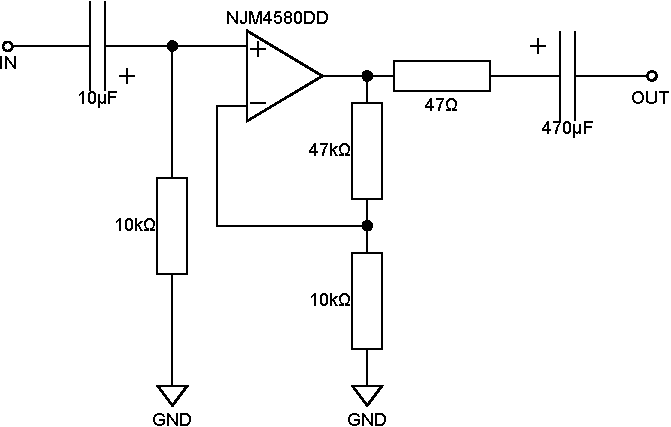
\includegraphics[width=13cm]{fig/amp.pdf}
	\caption{増幅回路}
	\label{fig:amplifier-circuit}
\end{figure}

\end{document}
